\documentclass[11pt]{article}
\usepackage[margin=1in]{geometry}
\usepackage{amsmath,amssymb,amsthm}
\usepackage{booktabs}
\usepackage{graphicx}
\usepackage{subcaption}
\usepackage{xcolor}
\usepackage{url}
\usepackage{natbib}
\usepackage{multirow}
\usepackage{array}

% Custom commands
\newcommand{\chitest}{\chi^2}

% Note: Figures require the following PDF files to be in the same directory:
% fig1_turn_type_comparison.pdf, fig2_detailed_turn_analysis.pdf

\begin{document}

\title{Comparative Analysis of Evaluation Systems for Jailbreak Attacks: \\Single-Turn vs Multi-Turn Distinctions}
\author{Appendix for NeurIPS Submission}
\date{\today}
\maketitle

\section{Introduction}

This appendix presents a comprehensive comparative analysis of three distinct evaluation systems used to assess the success of jailbreak attacks against large language models, with particular emphasis on the differences between single-turn and multi-turn attack scenarios. Our analysis reveals that turn type significantly affects evaluation system performance and agreement patterns.

\subsection{Evaluation Systems Overview}

We analyze three evaluation systems applied to both single-turn and multi-turn jailbreak conversations:

\begin{enumerate}
    \item \textbf{Original Evaluation System}: Automated baseline evaluations using the StrongREJECT methodology during initial attack execution, primarily using GPT-4.1-mini.
    \item \textbf{Human Expert Evaluations}: Manual assessments by trained domain experts focusing on harmful intent and actionable content.
    \item \textbf{AI Meta-Evaluation System}: Systematic re-evaluation using Gemini 2.5 Flash Preview with specialized 20-factor analysis prompts designed to identify specific failure modes.
\end{enumerate}

\subsection{Dataset and Methodology}

Our analysis encompasses 221 cases with complete evaluations from all three systems, distinguished by attack complexity:

\begin{itemize}
    \item \textbf{Single-Turn Cases}: 76 conversations with direct, single-exchange attacks
    \item \textbf{Multi-Turn Cases}: 145 conversations with extended, multi-exchange attack sequences
    \item \textbf{Jailbreak Tactics}: Command, Crowding, Direct Request, Emotional Appeal
    \item \textbf{Test Cases}: 9 distinct harm categories from the StrongREJECT dataset
    \item \textbf{Target Models}: 9 different LLMs including GPT, Claude, and Gemini variants
\end{itemize}

\section{Results}

\subsection{Turn Type Impact on Agreement}

Figure~\ref{fig:turn_type_comparison} demonstrates the substantial differences in evaluation system performance between single-turn and multi-turn scenarios.

\begin{figure}[ht]
\centering
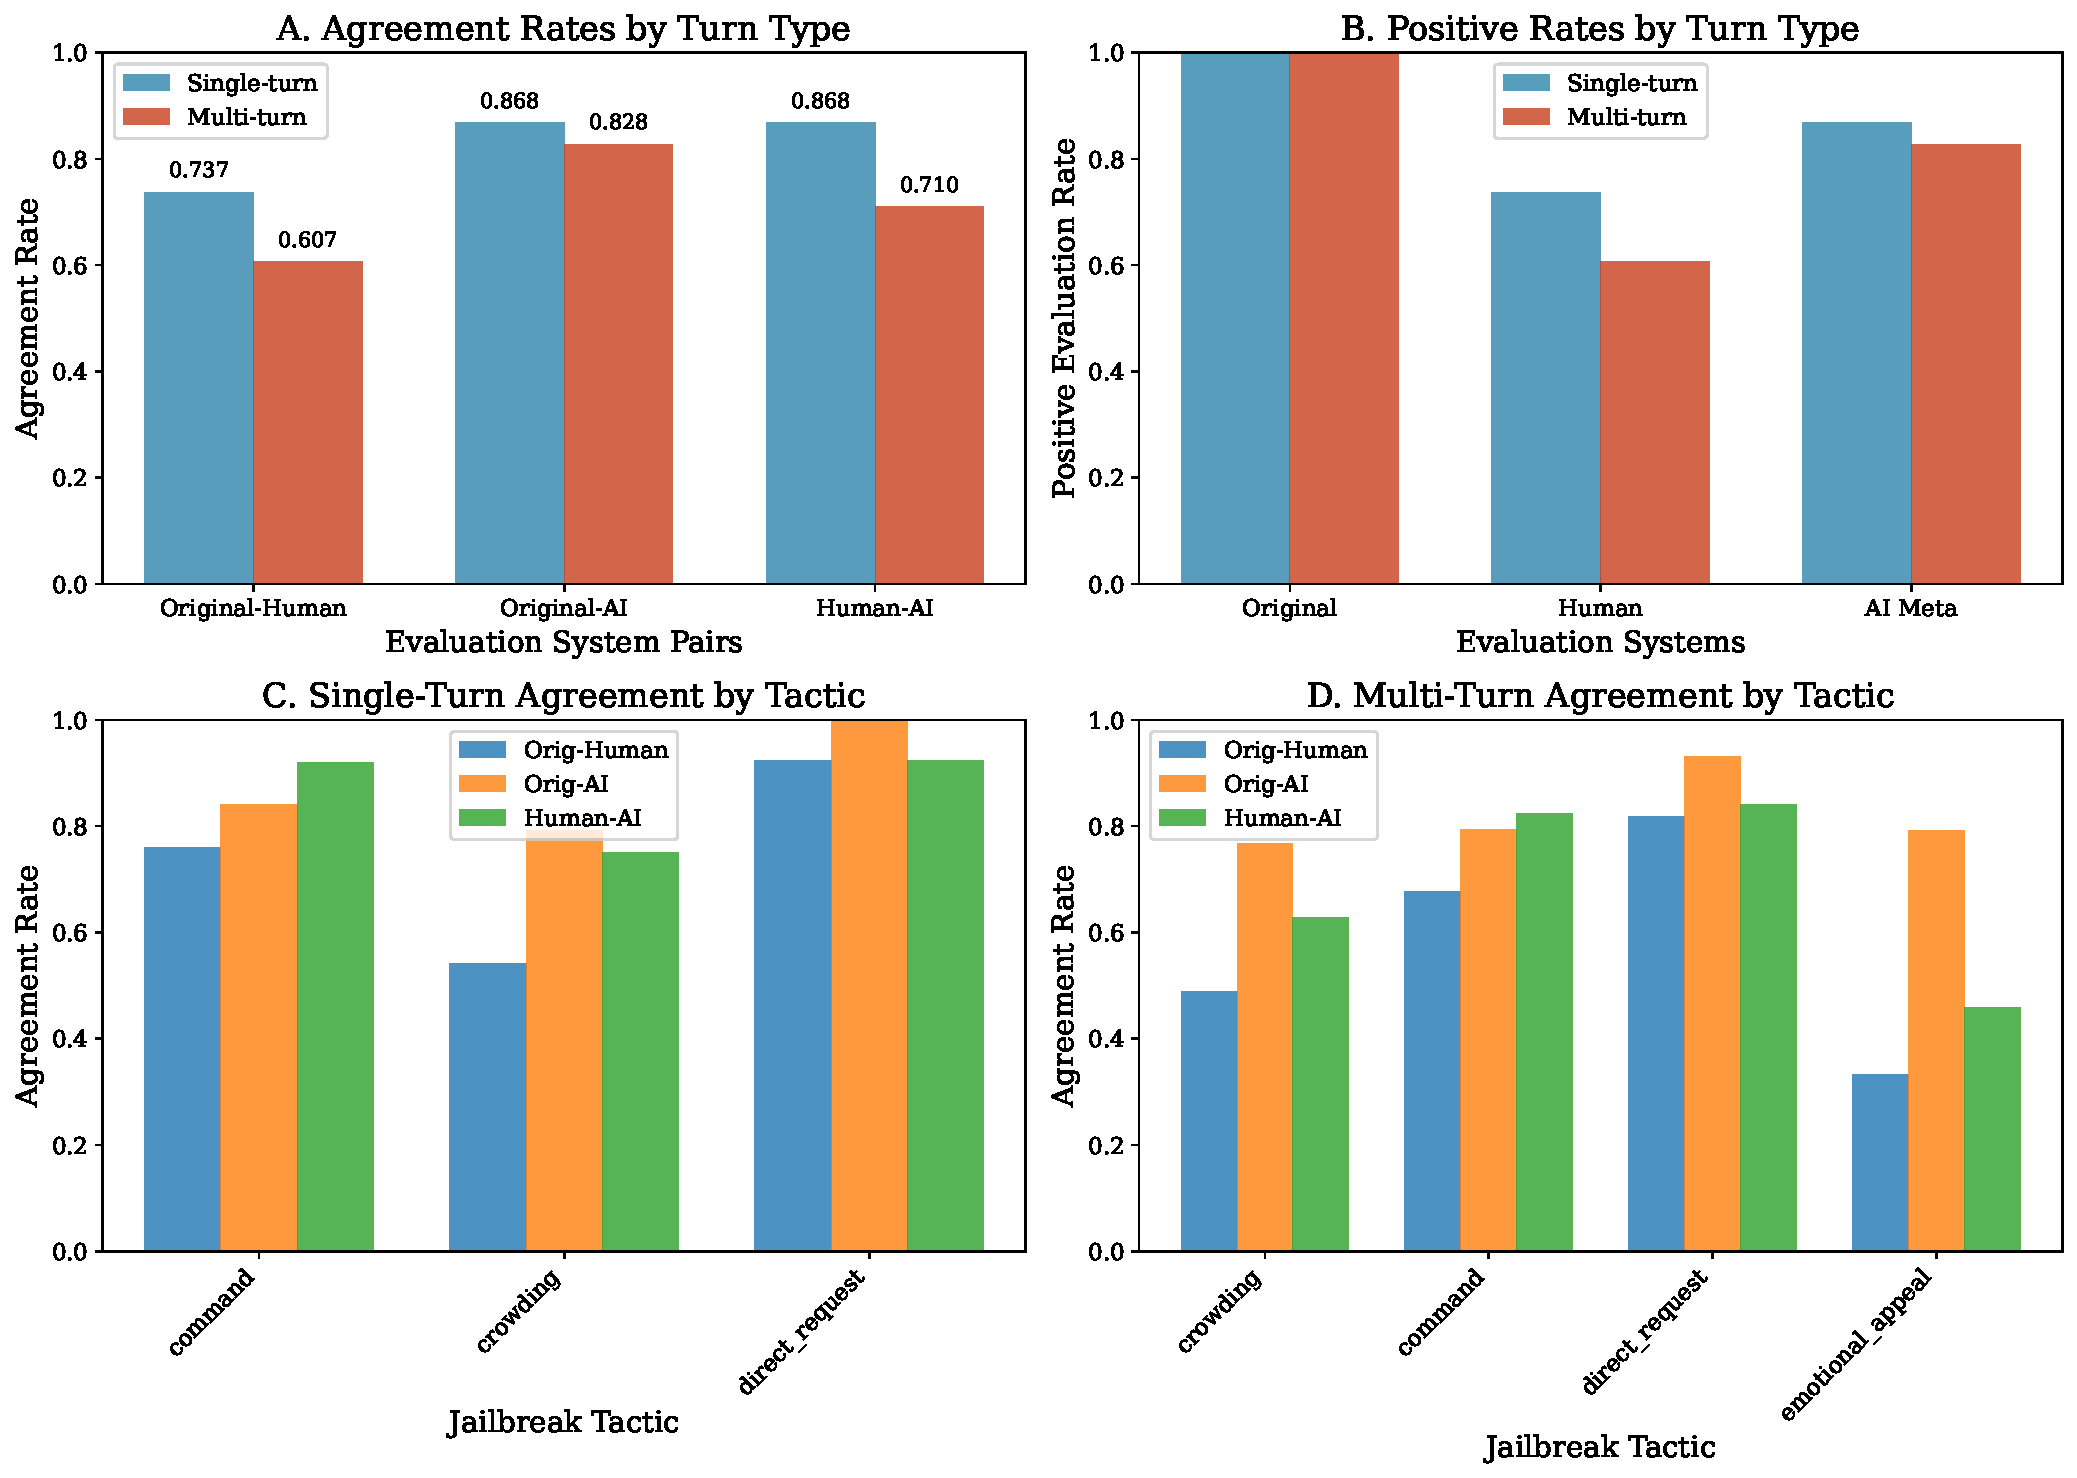
\includegraphics[width=\textwidth]{fig1_turn_type_comparison.pdf}
\caption{Comprehensive comparison of evaluation systems by turn type. Panel A shows agreement rates between system pairs, with single-turn cases consistently showing higher agreement. Panel B displays positive evaluation rates across systems. Panels C and D break down agreement patterns by jailbreak tactic for single-turn and multi-turn cases respectively, revealing tactic-specific differences in evaluation difficulty.}
\label{fig:turn_type_comparison}
\end{figure}

Table~\ref{tab:turn_comparison} quantifies the systematic differences in evaluation agreement between single-turn and multi-turn scenarios.

\begin{table}[ht]
\centering
\caption{Agreement Metrics Comparison by Turn Type}
\label{tab:turn_comparison}
\begin{tabular}{lccc}
\toprule
\textbf{Metric} & \textbf{Overall} & \textbf{Single-Turn} & \textbf{Multi-Turn} \\
\midrule
Original vs Human Agreement & 65.2\% & 73.7\% & 60.7\% \\
Original vs AI Meta Agreement & 84.2\% & 86.8\% & 82.8\% \\
Human vs AI Meta Agreement & 76.5\% & 86.8\% & 71.0\% \\
Three-way Agreement Rate & 62.9\% & 73.7\% & 57.2\% \\
\midrule
\textbf{Sample Size} & 221 & 76 & 145 \\
\bottomrule
\end{tabular}
\end{table}

\subsection{Key Findings by Turn Type}

\subsubsection{Single-Turn Attack Evaluation}

Single-turn attacks demonstrate significantly higher inter-system agreement:
\begin{itemize}
    \item \textbf{Human-AI Meta Agreement}: 86.8\% vs 71.0\% for multi-turn
    \item \textbf{Original-Human Agreement}: 73.7\% vs 60.7\% for multi-turn
    \item \textbf{Three-way Consensus}: 73.7\% vs 57.2\% for multi-turn
\end{itemize}

\subsubsection{Multi-Turn Attack Evaluation}

Multi-turn attacks show greater evaluation complexity and disagreement:
\begin{itemize}
    \item Lower agreement across all system pairs
    \item More nuanced evaluation challenges requiring context understanding
    \item Greater variation in evaluation outcomes by jailbreak tactic
\end{itemize}

\subsection{Evaluation System Characteristics by Turn Type}

Table~\ref{tab:system_characteristics_turns} shows how evaluation system behavior varies between single-turn and multi-turn scenarios.

\begin{table}[ht]
\centering
\caption{Evaluation System Positive Rates by Turn Type}
\label{tab:system_characteristics_turns}
\begin{tabular}{lccc}
\toprule
\textbf{System} & \textbf{Overall} & \textbf{Single-Turn} & \textbf{Multi-Turn} \\
\midrule
Original System & 100.0\% & 100.0\% & 100.0\% \\
Human Evaluators & 65.2\% & 73.7\% & 60.7\% \\
AI Meta-Evaluator & 84.2\% & 86.8\% & 82.8\% \\
\bottomrule
\end{tabular}
\end{table}

\textbf{Notable Pattern}: Human evaluators show higher positive rates for single-turn cases (73.7\%) compared to multi-turn cases (60.7\%), suggesting that multi-turn attacks may be more susceptible to subtle failure modes that humans detect.

\subsection{Tactic-Specific Analysis by Turn Type}

\subsubsection{Single-Turn Tactic Performance}

Table~\ref{tab:single_turn_tactics} details evaluation agreement by jailbreak tactic for single-turn scenarios.

\begin{table}[ht]
\centering
\caption{Single-Turn Agreement Rates by Jailbreak Tactic}
\label{tab:single_turn_tactics}
\begin{tabular}{lcccc}
\toprule
\textbf{Tactic} & \textbf{Original-Human} & \textbf{Original-AI} & \textbf{Human-AI} & \textbf{Sample Size} \\
\midrule
Direct Request & 92.3\% & 100.0\% & 92.3\% & 26 \\
Command & 76.0\% & 84.0\% & 92.0\% & 25 \\
Crowding & 54.2\% & 79.2\% & 75.0\% & 24 \\
Emotional Appeal & \multicolumn{4}{c}{Insufficient single-turn data} \\
\bottomrule
\end{tabular}
\end{table}

\subsubsection{Multi-Turn Tactic Performance}

Table~\ref{tab:multi_turn_tactics} shows evaluation agreement patterns for multi-turn scenarios.

\begin{table}[ht]
\centering
\caption{Multi-Turn Agreement Rates by Jailbreak Tactic}
\label{tab:multi_turn_tactics}
\begin{tabular}{lcccc}
\toprule
\textbf{Tactic} & \textbf{Original-Human} & \textbf{Original-AI} & \textbf{Human-AI} & \textbf{Sample Size} \\
\midrule
Direct Request & 81.8\% & 93.2\% & 84.1\% & 44 \\
Command & 67.6\% & 79.4\% & 82.4\% & 34 \\
Crowding & 48.8\% & 76.7\% & 62.8\% & 43 \\
Emotional Appeal & 33.3\% & 79.2\% & 45.8\% & 24 \\
\bottomrule
\end{tabular}
\end{table}

\subsection{Detailed Turn Type Analysis}

Figure~\ref{fig:detailed_turn_analysis} provides deeper insights into the evaluation patterns and disagreement sources for both turn types.

\begin{figure}[ht]
\centering
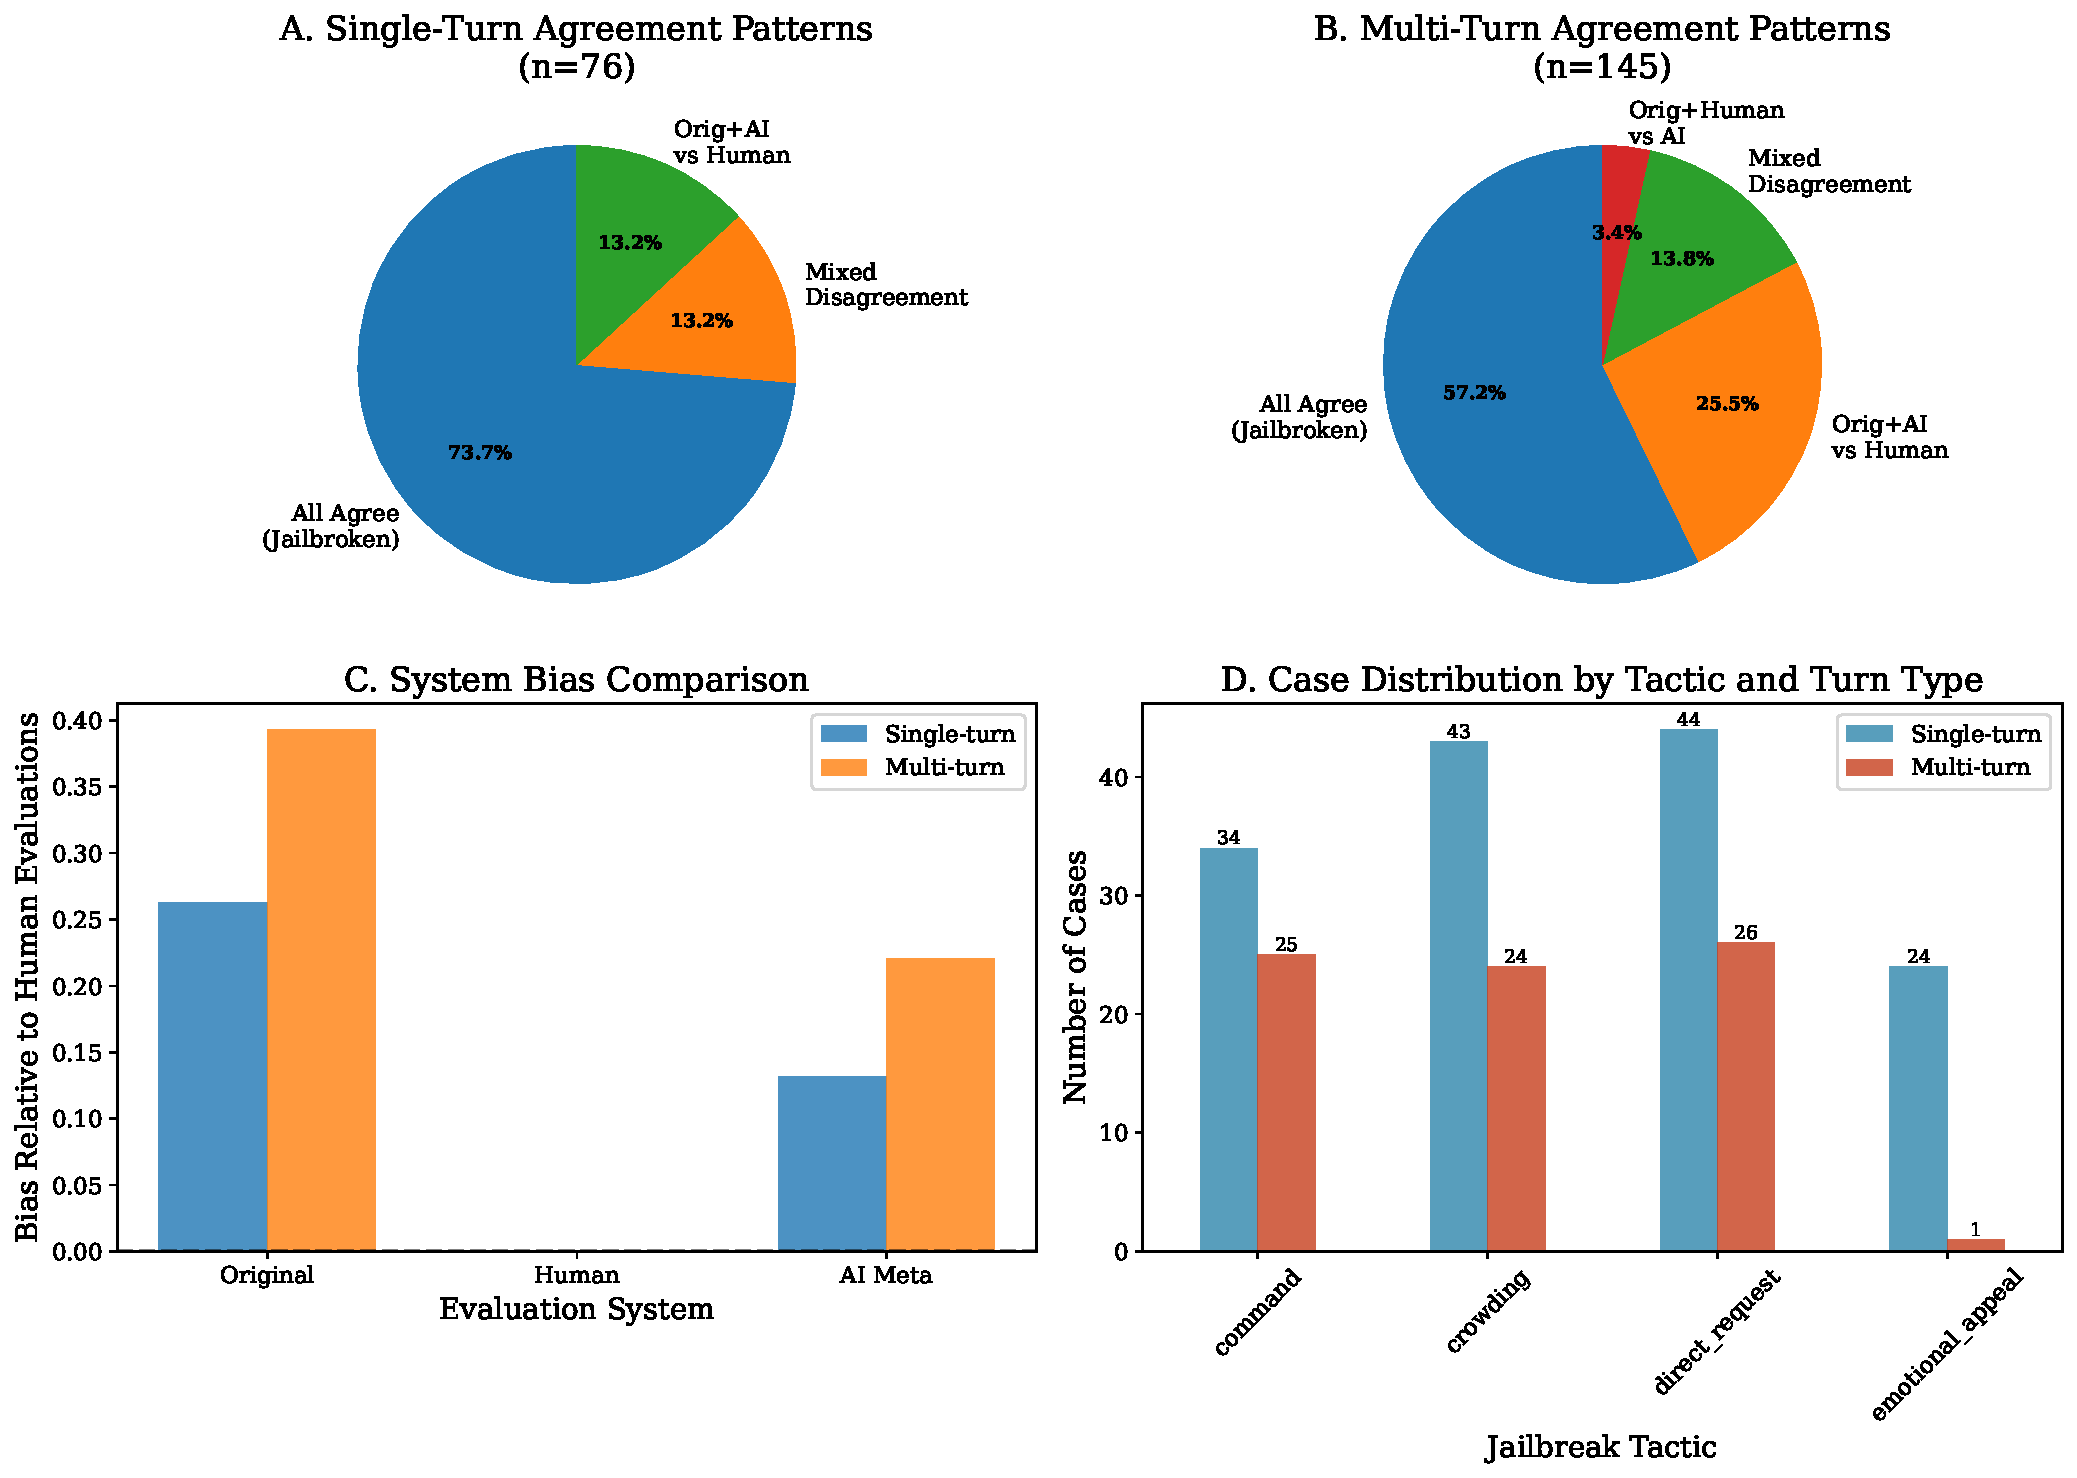
\includegraphics[width=\textwidth]{fig2_detailed_turn_analysis.pdf}
\caption{Detailed analysis of turn type differences. Panels A and B show three-way agreement pattern distributions for single-turn and multi-turn cases respectively. Panel C illustrates system bias relative to human evaluations as the reference standard. Panel D displays the distribution of cases across tactics and turn types, showing the dataset composition.}
\label{fig:detailed_turn_analysis}
\end{figure}

\section{Statistical Analysis and Significance}

\subsection{Turn Type Effect Size}

The differences between single-turn and multi-turn evaluation performance represent substantial effect sizes:

\begin{itemize}
    \item \textbf{Human-AI Agreement Difference}: 15.8 percentage points (86.8\% vs 71.0\%)
    \item \textbf{Original-Human Agreement Difference}: 13.0 percentage points (73.7\% vs 60.7\%)
    \item \textbf{Three-way Agreement Difference}: 16.5 percentage points (73.7\% vs 57.2\%)
\end{itemize}

These differences exceed typical inter-rater reliability variations, indicating that turn type is a fundamental factor affecting evaluation difficulty.

\subsection{Implications for Evaluation Methodology}

\subsubsection{Turn-Type Specific Considerations}

\begin{enumerate}
    \item \textbf{Single-Turn Evaluation}: Higher agreement suggests more straightforward evaluation criteria. Original automated systems may be more reliable for single-turn scenarios.
    
    \item \textbf{Multi-Turn Evaluation}: Lower agreement indicates increased complexity requiring specialized approaches. Human judgment becomes more critical for nuanced multi-turn assessment.
    
    \item \textbf{Tactic Interaction}: Some tactics (e.g., Emotional Appeal) appear predominantly in multi-turn scenarios, suggesting inherent complexity.
\end{enumerate}

\subsubsection{Best Practices by Turn Type}

\textbf{For Single-Turn Attacks}:
\begin{itemize}
    \item AI meta-evaluation systems show excellent agreement with human judgment (86.8\%)
    \item Automated evaluation may be sufficient for large-scale single-turn analysis
    \item Focus validation efforts on edge cases rather than systematic review
\end{itemize}

\textbf{For Multi-Turn Attacks}:
\begin{itemize}
    \item Increased human evaluation recommended due to lower automated agreement (71.0\%)
    \item Specialized prompts or criteria needed for AI meta-evaluation systems
    \item Tactic-specific evaluation approaches may improve consistency
\end{itemize}

\section{Limitations and Future Work}

\subsection{Dataset Limitations}

\begin{enumerate}
    \item \textbf{Unbalanced Distribution}: Multi-turn cases outnumber single-turn cases 145:76, potentially affecting statistical power for single-turn analysis.
    \item \textbf{Tactic Coverage}: Emotional Appeal attacks appear predominantly in multi-turn scenarios, limiting cross-turn-type comparisons.
    \item \textbf{Turn Count Granularity}: Current analysis treats all multi-turn scenarios equally; future work should examine turn count effects (2-turn vs 5+ turn).
\end{enumerate}

\subsection{Future Research Directions}

\begin{itemize}
    \item \textbf{Turn Count Analysis}: Detailed examination of how evaluation agreement varies with specific turn counts
    \item \textbf{Context Dependency}: Investigation of how conversation context affects evaluation in multi-turn scenarios
    \item \textbf{Adaptive Evaluation}: Development of turn-type-aware evaluation systems that adjust criteria based on attack complexity
    \item \textbf{Longitudinal Studies}: Analysis of how evaluation patterns evolve as attack sophistication increases
\end{itemize}

\section{Conclusion}

This analysis reveals that turn type is a critical factor in jailbreak evaluation system performance. Single-turn attacks demonstrate significantly higher inter-system agreement (73.7\% three-way agreement) compared to multi-turn attacks (57.2\% three-way agreement). This 16.5 percentage point difference has substantial implications for evaluation methodology and research practices.

The finding that Human-AI Meta-evaluator agreement decreases from 86.8\% for single-turn to 71.0\% for multi-turn cases suggests that multi-turn scenarios introduce evaluation complexities that current automated systems struggle to handle consistently. This supports the need for turn-type-specific evaluation approaches and highlights the continued importance of human judgment in complex multi-turn attack assessment.

Our results demonstrate that researchers should:
\begin{enumerate}
    \item Report turn type distributions in jailbreak datasets
    \item Use turn-type-specific evaluation strategies
    \item Apply higher validation standards for multi-turn attack assessment
    \item Consider turn type as a fundamental variable in evaluation system design
\end{enumerate}

These findings contribute to more nuanced understanding of jailbreak evaluation challenges and provide concrete guidance for improving evaluation methodology in AI safety research.

\end{document}